\documentclass{article}

\usepackage{algorithm}
\usepackage{algorithmic}
\usepackage{graphicx}
\usepackage{marvosym}
\usepackage{dingbat}
\usepackage{tikz}

\title{Linked list traversal}
\date{07/12/2015}

\usetikzlibrary{arrows}

\tikzset{
  treenode/.style = {align=center, inner sep=0pt, text centered, font=\sffamily},
  wn/.style = {treenode, circle, black, font=\ttfamily, draw=white, fill=white, text width=1.5em},
  txt/.style = {black, anchor=west, font=\ttfamily, draw=white, fill=white},
  edge from parent/.style={thick,draw=black, latex-}
}

\begin{document}
\maketitle

\section{Binary tree traversal}

This exercise is about parallelizing the traversal of a postordered
binary tree.

The tree is described by two integers and three arrays:

\begin{itemize}
\item \texttt{l}: the number of levels in the tree.
\item \texttt{n}: the number of nodes in the tree. Note that
  $n=2^l-1$.
\item \texttt{*data}: \texttt{data[i]} contains an integer data
  associated with node \texttt{i}.
\item \texttt{*left}: \texttt{left[i]} is the index of the left child
  of node \texttt{i}.
\item \texttt{*right}: \texttt{right[i]} is the index of the right child
  of node \texttt{i}.
\end{itemize}

Nodes are numbered from $0$ to $n-1$ in post-order: this means that
all the nodes in a subtree are numbered consecutively. This implies
that a node of the tree has a index greater that all its descendants;
as a results, visiting the nodes in the natural order $0, 1, 2, ...$
implies that a node is always visited after its children. Here is an
example of binary tree with the corresponding data structure:

\vspace{0.5cm}

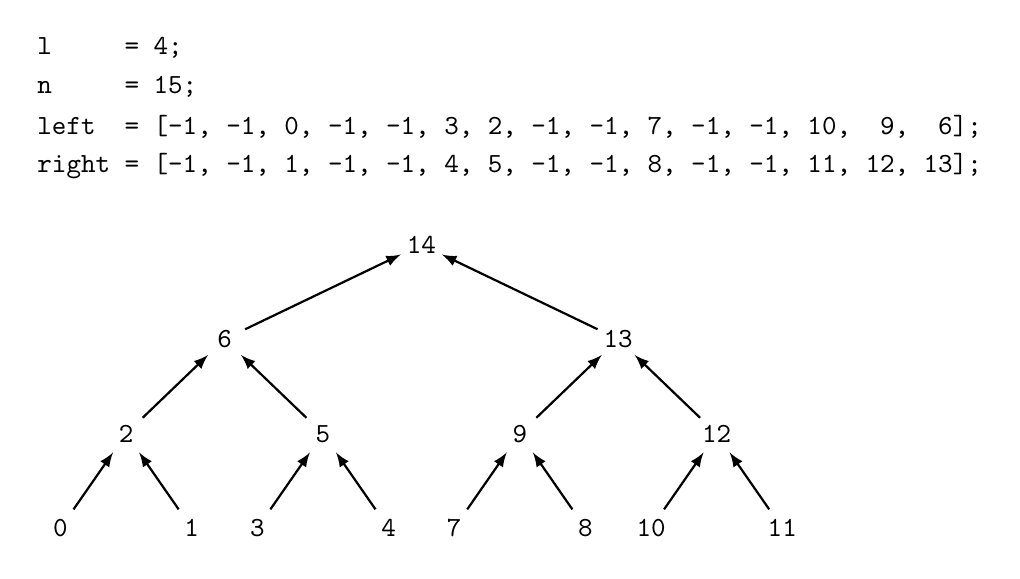
\begin{tikzpicture}[->,>=stealth',level/.style={sibling distance = 5cm/#1,
  level distance = 1.2cm}] 

\node [txt] at (-5,2.5) {l~~~~~= 4;};
\node [txt] at (-5,2.0) {n~~~~~= 15;};
\node [txt] at (-5,1.5) {left~~= [-1, -1, 0, -1, -1, 3, 2, -1, -1, 7, -1, -1, 10, ~9, ~6];};
\node [txt] at (-5,1.0) {right~= [-1, -1, 1, -1, -1, 4, 5, -1, -1, 8, -1, -1, 11, 12, 13];};

\node [wn] at (0,0) {14}
child{ node [wn] {6} 
  child{ node [wn] {2} 
    child{ node [wn] {0}} 
    child{ node [wn] {1}}
  }
  child{ node [wn] {5}
    child{ node [wn] {3}}
    child{ node [wn] {4}}
  }                            
}
child{ node [wn] {13}
  child{ node [wn] {9} 
    child{ node [wn] {7}}
    child{ node [wn] {8}}
  }
  child{ node [wn] {12}
    child{ node [wn] {10}}
    child{ node [wn] {11}}
  }
}; 
\end{tikzpicture}

Note that both \texttt{left[i]} and \texttt{right[i]} are equal to
$-1$ for a leaf node.

The following code is used to traverse the tree and compute, for each
node a data, \texttt{data[i]} by combining the index of the node
\texttt{i}, and the data computed on its left and right children:

\begin{verbatim}
  for(i=0; i<n; i++){
    l = left[i];
    r = right[i];
    data[i] = process(data[l], data[r], i);
  }
\end{verbatim}



\section{Package content}
In the \texttt{tree\_traversal} directory you will find the
following files:
\begin{itemize}
\item \texttt{main.c}: this file contains the main program which first
  initializes the tree for a provided number of levels. The main
  program then calls a sequential routine \texttt{treetrav\_seq}
  containing the code above, then reinitializes the tree and call the
  \texttt{treetrav\_par} routine which is supposed to contain a
  parallel version of the traversal code.
\item \texttt{treetrav\_seq.c}: contains a routine implementing a
  sequential traversal with the code presented above.
\item \texttt{treetrav\_par.c} contains a routine implementing a
  parallel tree traversal. \textbf{Only this file has to be modified
    for this exercise}.
\item \texttt{aux.c, aux.h}: these two files contain auxiliary
  routines and \textbf{must not be modified}.
\end{itemize}



The code can be compiled with the \texttt{make} command: just type
\texttt{make} inside the \texttt{tree\_traversal} directory; this
will generate a \texttt{main} program that can be run like this:

\begin{verbatim}
$ ./main l
\end{verbatim}

where \texttt{l} is the number of levels in the tree.

\section{Assignment}
\begin{itemize}
\item {\huge \Keyboard} At the beginning, the \texttt{treetrav\_par}
  routine contains an exact copy of the \texttt{treetrav\_seq}
  one. Modify these routine in order to parallelize it using the
  OpenMP \texttt{task} construct.
  Make sure that the result computed by the three routines (sequential
  and parallel ones) is consistently (that is, at every execution of
  the parallel code) the same; a message printed at the end of the
  execution will tell you whether this is the case.
\item \smallpencil Report the execution times for the implemented
  parallel version with 1, 2 and 4 threads and for different tree
  sizes. Analyze and comment on your results: is the achieved speedup
  reasonable or not?. Report your answer in the \texttt{responses.txt}
  file.
\end{itemize}


\paragraph{Advice}
\begin{itemize}
\item When using the OpenMP \texttt{task} construct, always think
  about data scoping to make sure input data has the correct
  value upon execution of the task and returned results do not go out
  of scope when the task is finished.
\end{itemize}



















\end{document}




%%% Local Variables: 
%%% mode: latex
%%% TeX-master: t
%%% End: 
